% Options for packages loaded elsewhere
\PassOptionsToPackage{unicode}{hyperref}
\PassOptionsToPackage{hyphens}{url}
%
\documentclass[
  ignorenonframetext,
]{beamer}
\usepackage{pgfpages}
\setbeamertemplate{caption}[numbered]
\setbeamertemplate{caption label separator}{: }
\setbeamercolor{caption name}{fg=normal text.fg}
\beamertemplatenavigationsymbolsempty
% Prevent slide breaks in the middle of a paragraph
\widowpenalties 1 10000
\raggedbottom
\setbeamertemplate{part page}{
  \centering
  \begin{beamercolorbox}[sep=16pt,center]{part title}
    \usebeamerfont{part title}\insertpart\par
  \end{beamercolorbox}
}
\setbeamertemplate{section page}{
  \centering
  \begin{beamercolorbox}[sep=12pt,center]{part title}
    \usebeamerfont{section title}\insertsection\par
  \end{beamercolorbox}
}
\setbeamertemplate{subsection page}{
  \centering
  \begin{beamercolorbox}[sep=8pt,center]{part title}
    \usebeamerfont{subsection title}\insertsubsection\par
  \end{beamercolorbox}
}
\AtBeginPart{
  \frame{\partpage}
}
\AtBeginSection{
  \ifbibliography
  \else
    \frame{\sectionpage}
  \fi
}
\AtBeginSubsection{
  \frame{\subsectionpage}
}
\usepackage{lmodern}
\usepackage{amssymb,amsmath}
\usepackage{ifxetex,ifluatex}
\ifnum 0\ifxetex 1\fi\ifluatex 1\fi=0 % if pdftex
  \usepackage[T1]{fontenc}
  \usepackage[utf8]{inputenc}
  \usepackage{textcomp} % provide euro and other symbols
\else % if luatex or xetex
  \usepackage{unicode-math}
  \defaultfontfeatures{Scale=MatchLowercase}
  \defaultfontfeatures[\rmfamily]{Ligatures=TeX,Scale=1}
\fi
\usecolortheme{seahorse}
% Use upquote if available, for straight quotes in verbatim environments
\IfFileExists{upquote.sty}{\usepackage{upquote}}{}
\IfFileExists{microtype.sty}{% use microtype if available
  \usepackage[]{microtype}
  \UseMicrotypeSet[protrusion]{basicmath} % disable protrusion for tt fonts
}{}
\makeatletter
\@ifundefined{KOMAClassName}{% if non-KOMA class
  \IfFileExists{parskip.sty}{%
    \usepackage{parskip}
  }{% else
    \setlength{\parindent}{0pt}
    \setlength{\parskip}{6pt plus 2pt minus 1pt}}
}{% if KOMA class
  \KOMAoptions{parskip=half}}
\makeatother
\usepackage{xcolor}
\IfFileExists{xurl.sty}{\usepackage{xurl}}{} % add URL line breaks if available
\IfFileExists{bookmark.sty}{\usepackage{bookmark}}{\usepackage{hyperref}}
\hypersetup{
  hidelinks,
  pdfcreator={LaTeX via pandoc}}
\urlstyle{same} % disable monospaced font for URLs
\newif\ifbibliography
\setlength{\emergencystretch}{3em} % prevent overfull lines
\providecommand{\tightlist}{%
  \setlength{\itemsep}{0pt}\setlength{\parskip}{0pt}}
\setcounter{secnumdepth}{-\maxdimen} % remove section numbering
\usepackage{luatexja-otf}
\hypersetup{unicode=true}
\usepackage{luatexja-fontspec}
\setmainjfont[BoldFont=HaranoAjiGothic-Bold]{HaranoAjiGothic-Regular}
\setsansjfont{HaranoAjiGothic-Medium}
\usepackage{setspace}
\newcommand{\bdoublespace}{\begin{spacing}{1.5}}
\newcommand{\edoublespace}{\end{spacing}{}}
\newcommand{\vspacelarge}{\vspace{6mm}}
\newcommand{\vspacesmall}{\vspace{3mm}}
\setbeamertemplate{navigation symbols}{}
\setbeamertemplate{footline}[page number]
\setbeamertemplate{itemize items}[circle]

\title{Chapter 1\\
Nothing as Practical as a Good Theory\\
良い理論ほど実際に役に立つものはない}
\subtitle{in "Fish Ecology, Evolution, and Exploitation:\\
A Theoretical Synthesis"\\
by Ken H. Andersen}
\author{担当:西嶋 翔太\\
(中央水産研究所)}
\date{2020-05-11}

\begin{document}
\frame{\titlepage}

\begin{frame}{著者について \footnote[frame]{https://ken.haste.dk/}}
\protect\hypertarget{ux8457ux8005ux306bux3064ux3044ux3066}{}

\begin{block}{Ken H. Andersen}

\begin{columns}
\column{0.30\textwidth}


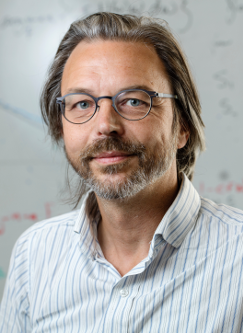
\includegraphics[width=100px]{KenAndersen} 

\column{0.70\textwidth}

I want to understand how life in the ocean is organised, why marine organisms look and act the way they do, and how marine ecosystems react to perturbations like  fishing, species removals/invasions or climate change.  
  
\vspacesmall
More specifically I work on:  

- Trait-based models of life in the ocean  

- Size-structured models of marine ecosystems  

- Fisheries induced  evolution  
  
\vspacesmall
Previously I have worked with sand ripples under surface waves and barchan dunes in deserts.

\end{columns}

\end{block}

\end{frame}

\begin{frame}{Google Scholar Citation}
\protect\hypertarget{google-scholar-citation}{}

\begin{center}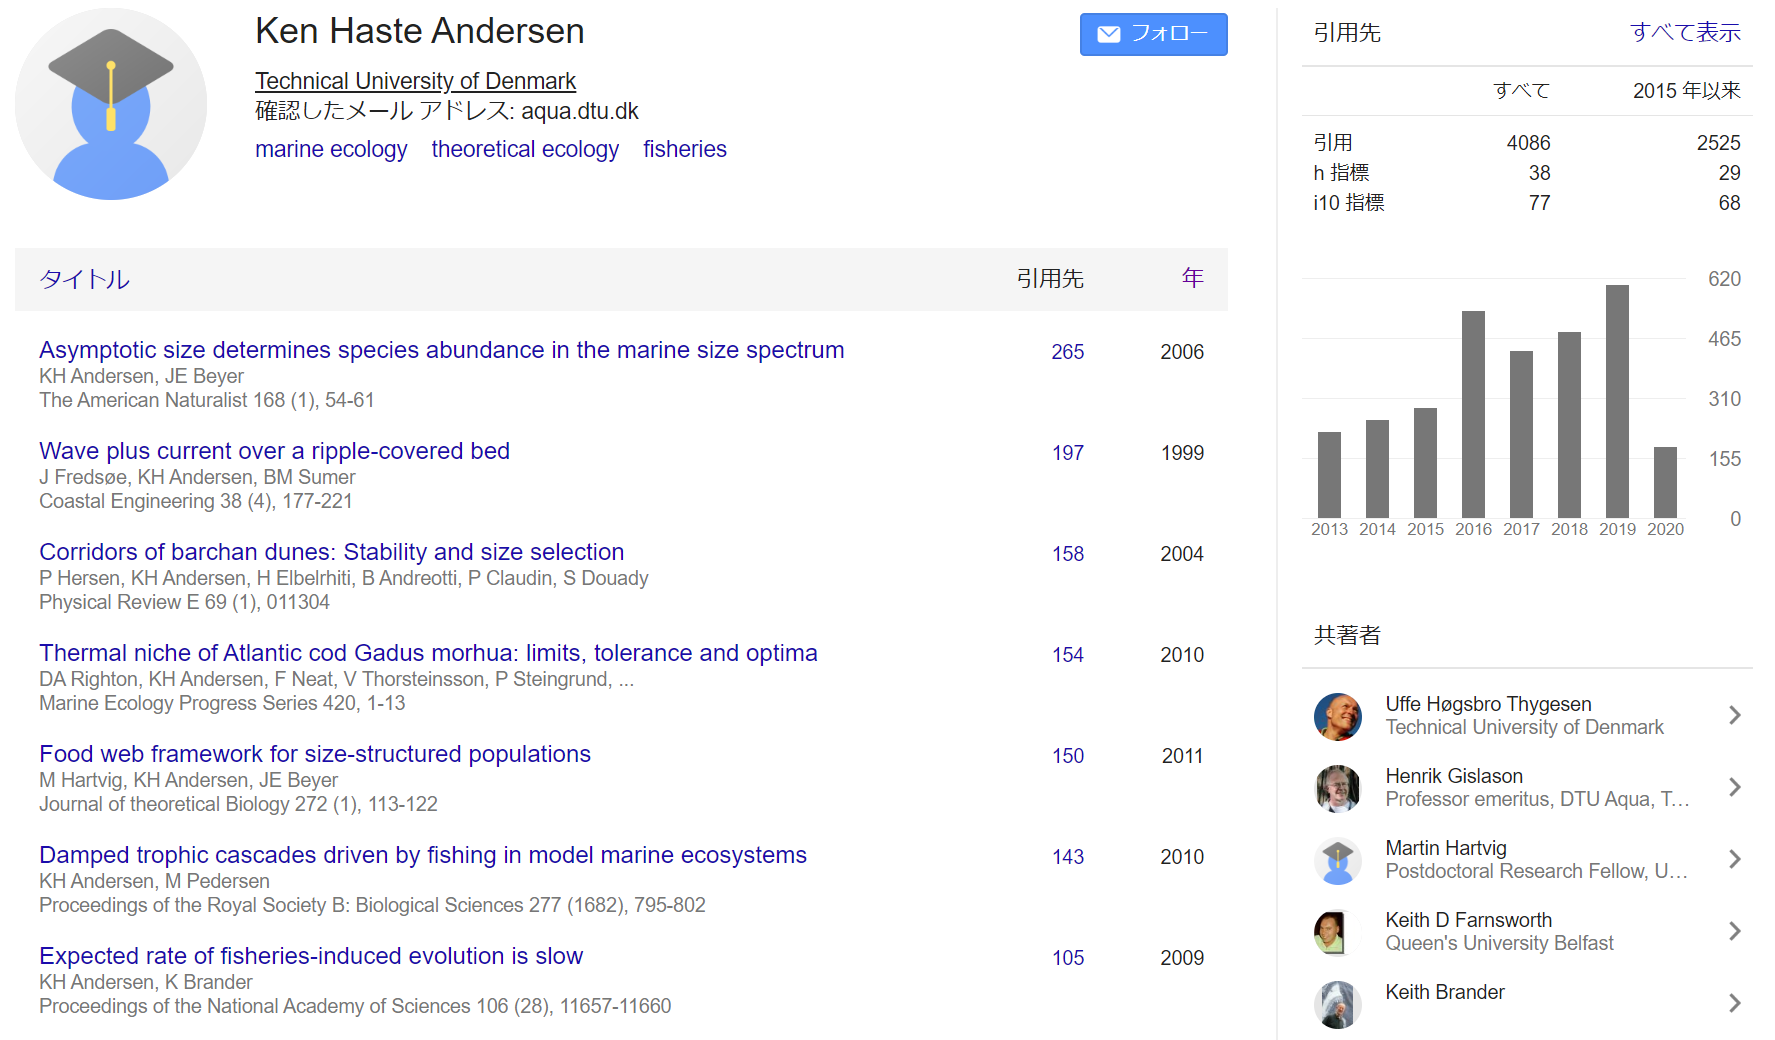
\includegraphics[width=1.05\linewidth]{GoogleScholarCitation} \end{center}

\end{frame}

\begin{frame}{この本のレビュー
\footnote[frame]{https://press.princeton.edu/books/hardcover/9780691176550/fish-ecology-evolution-and-exploitation}}
\protect\hypertarget{ux3053ux306eux672cux306eux30ecux30d3ux30e5ux30fc}{}

\begin{columns}
\column{0.25\textwidth}


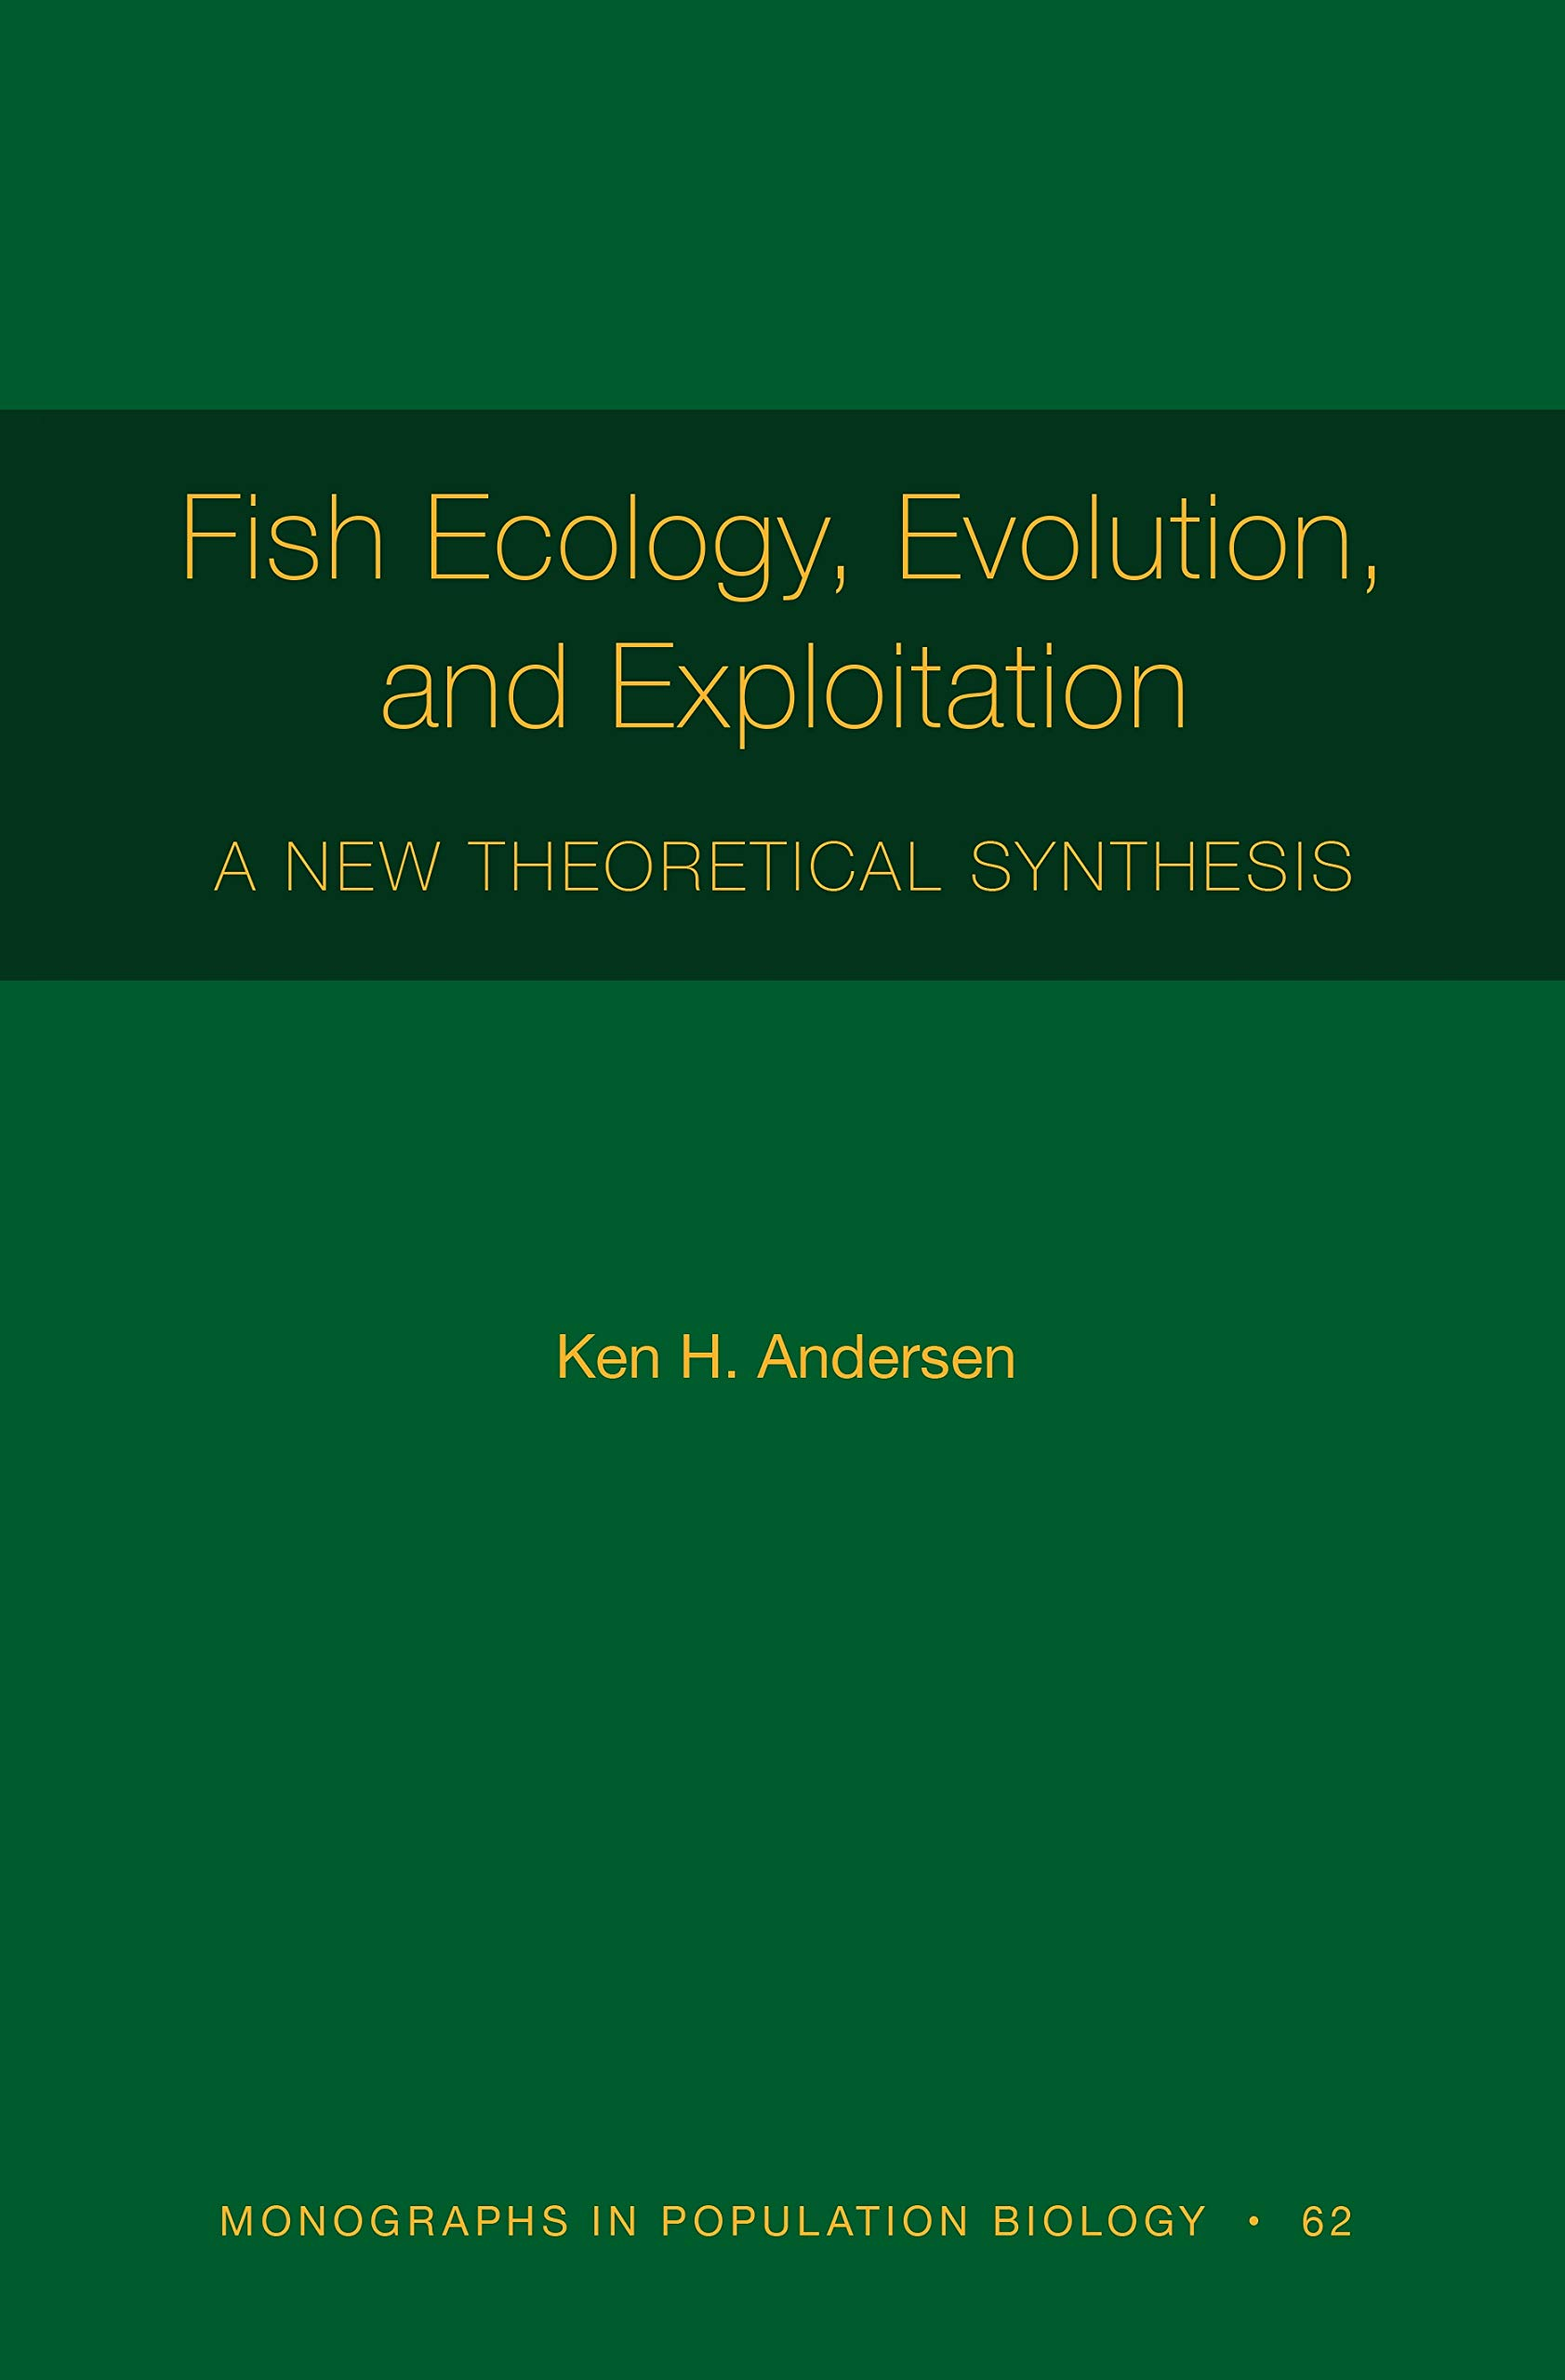
\includegraphics[width=80px]{FishEcoEvoBook} 

\column{0.75\textwidth}

- "Andersen pulls together a cohesive theory from a synthesis of decades of work. He presents a clear and pragmatic foundation for understanding the dynamics at the heart of fisheries and ecology—of individuals, populations, and communities. This leveler will help pave the way for many to tackle the leviathan that is multispecies fisheries."—Beth Fulton\pause

\vspacesmall
- "This book is a fantastic explanation of size- and trait-based analysis of marine ecosystems that should be required reading for marine ecologists and fisheries scientists. Among other results, Andersen provides insights into a community-based approach to ecosystem-based fisheries management."—Ray Hilborn

\end{columns}

\end{frame}

\begin{frame}

\begin{LARGE} 
\begin{center}
\begin{bf}
Chapter 1  
  
Nothing as Practical as a Good Theory
\end{bf}
\end{center}
\end{LARGE}

\end{frame}

\begin{frame}{魚の漁業管理の現状}
\protect\hypertarget{ux9b5aux306eux6f01ux696dux7ba1ux7406ux306eux73feux72b6}{}

\begin{itemize}
\tightlist
\item
  魚は約1gから100kgまでの体サイズをもち、海の優占的な生物\\
  \vspacelarge
\item
  生産性は高く、人々の食糧と富の供給源\\
  \vspacelarge
\item
  水産業は世界のたんぱく質の消費量の10%を供給し、その価値は100億ドル
  (FAO 2016)\\
  \vspacelarge
\item
  20世紀半ばに近代トロールの技術が登場して以来、魚類資源の過剰利用が可能になった\\
  \vspacelarge
\item
  高い漁獲量を維持するためには、漁業管理が必要である
\end{itemize}

\end{frame}

\begin{frame}{Beverton and Holt}
\protect\hypertarget{beverton-and-holt}{}

漁業管理勧告の多くはべバートン・ホルトの枠組みに基づいており、老朽化している

\begin{center}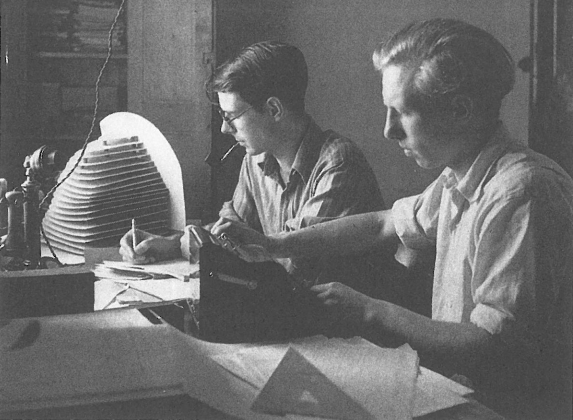
\includegraphics[width=250px]{Fig1} \end{center}

\end{frame}

\begin{frame}{漁業管理が直面している課題と疑問}
\protect\hypertarget{ux6f01ux696dux7ba1ux7406ux304cux76f4ux9762ux3057ux3066ux3044ux308bux8ab2ux984cux3068ux7591ux554f}{}

\begin{itemize}
\tightlist
\item
  単一資源管理から生態系アプローチへの拡張\\
  \vspacelarge
\item
  漁業による選択の長期的な進化的影響は?\\
  \vspacelarge
\item
  生物宅的情報が(ほとんど)ない状況、特に開発途上国において、多くの割合を占める「データ不足
  (data poor)」な資源をどう管理すべきか?\\
  \vspacelarge
\item
  種の多様性が高く、種をほとんど区別しない漁業が実施されており、資源毎の管理が非現実的な多くの生態系をどう扱うべきか?
\end{itemize}

\end{frame}

\begin{frame}{水産資源学と一般生態学}
\protect\hypertarget{ux6c34ux7523ux8cc7ux6e90ux5b66ux3068ux4e00ux822cux751fux614bux5b66}{}

\begin{itemize}
\tightlist
\item
  手助けやインスピレーションの基となるのは(一般)生態学である\\
  \vspacelarge
\item
  べバートンとホルトがその枠組みを構築して以来、水産資源学は生態学からは分岐し、管理のための実践的な場面への適用に重きを置くようになった\\
  \vspacelarge
\item
  水産資源学は独自の会議や学会を発展させ、プロシーディングスや会議文書といったグレイペーパーや専門的な雑誌で研究発表を行ってきた\\
  \vspacelarge
\item
  一方で生態学は、陸水学・食物網生態学・構造のある個体群・進化生態学といった水産資源学にも関連する分野を発展させた
\end{itemize}

\end{frame}

\begin{frame}{関連分野における生態学の発展}
\protect\hypertarget{ux95a2ux9023ux5206ux91ceux306bux304aux3051ux308bux751fux614bux5b66ux306eux767aux5c55}{}

\begin{block}{陸水学}

\begin{itemize}
\tightlist
\item
  多様性が低く、生息地の構造が単純であるため、観察や理解が容易
\item
  構造をもつ個体群の消費者―資源動態の発展
\item
  漁業が行われていない海の状態に近い\pause
\end{itemize}

\end{block}

\begin{block}{食物網生態学}

\begin{itemize}
\tightlist
\item
  食物網構造と安定性の関係に着目し、普遍的なパターンを探求
\item
  漁業などの攪乱への応答は中心的な課題ではなかった\pause  
\end{itemize}

\end{block}

\begin{block}{進化生態学}

\begin{itemize}
\tightlist
\item
  ``Life history invariants''は魚類の観察から生まれた
\item
  子のサイズ戦略の多様性、繁殖戦略、不定成長の進化は魚類進化の中心的問い
\item
  魚類の生活史の理解が水産資源学にはあまり応用されていない
\end{itemize}

\end{block}

\end{frame}

\begin{frame}{この本の目的}
\protect\hypertarget{ux3053ux306eux672cux306eux76eeux7684}{}

\begin{itemize}
\tightlist
\item
  サイズベース・形質ベースのアプローチを、
  魚類の個体群と群集をモデリングするための近代的で一貫した統一的枠組みとして紹介する\\
  \vspacesmall
\item
  本理論は生態学と水産資源学の新しい発展から編み出されており、漁業と生態学の問題に幅広く適用可能である\\
  \vspacesmall
\item
  長期間放置されてきた、魚類生態学と水産資源学の思考の統一に貢献したい\\
  \vspacesmall
\item
  ここでは本理論の基本要素を説明するが、古典的な水産資源学に由来する要素から始めて、次に海洋生態学・生理学的に構造化した個体群モデル・形質生態学において発展したサイズベース理論を紹介する
\end{itemize}

\end{frame}

\begin{frame}{方針}
\protect\hypertarget{ux65b9ux91dd}{}

\begin{itemize}[<+->]
\tightlist
\item
  生態系アプローチを漁業管理に適用できるように、べバートン・ホルトの枠組みを修復し、欠けている要素を補うという誘惑に駆られるかもしれない\\
\item
  べバートン・ホルトの修復では、
  厳密な理論は構築できない(2つのバイクを溶接して自動車を作るようなものだ!)\\
\item
  漁業の勧告のような実践的な応用は、確固とした理論的・基礎的理解に基づくのがベストであるはず
  (この本のタイトルにある名言を作ったKurt Lewinと同様に)\\
\item
  Von
  Bertalanffyの成長式・スプレッドシートに適した生命表・親魚の死亡率\(M\)の概念を捨て,その代わりに生理学・微分方程式・サイズ依存の死亡率を使用する\\
\item
  本理論は、Hilborn \& Walters (1992) やQuinn \& Deriso
  (1999)といった古典に精通している人には取っつきにくく、複雑に感じるかもしれない\\
\item
  少ない仮定のみで、単一種の影響評価から進化率の推定や生態系の影響評価まで行えることが本理論の利点である
\end{itemize}

\end{frame}

\begin{frame}{多種系およびサイズベースのアプローチ}
\protect\hypertarget{ux591aux7a2eux7cfbux304aux3088ux3073ux30b5ux30a4ux30baux30d9ux30fcux30b9ux306eux30a2ux30d7ux30edux30fcux30c1}{}

\begin{itemize}[<+->]
\tightlist
\item
  Andersen(著者とは別人)とUrsinは1970年代に、「一次・二次生産から栄養塩循環、餌へのサイズ依存の選択性に至るまでのあらゆることは、魚1個体の生理的な描写に基づいている」という重要で新しい考えを紹介した
  (が、数式の複雑さや無名の雑誌で公表したことが原因で忘れ去られた)\\
\item
  著者の理論は、Kleiberの法則と呼ばれる体サイズによる代謝作用のスケーリングと「大きい魚はより小さい魚を食べる」という法則に基づく
\item
  この2つの法則は体サイズの分布を説明する (Sheldon et al.~1977) 
\item
  著者は群集だけでなく個体群内のサイズ分布も予測する 
\item
  WernerとGilliam (1984) は年齢ベースのべバートン・ホルト理論では
  異なるステージ間の競争や捕食を表すことができないと指摘し、
  体サイズに基づく理論的枠組みの草案を書いた\\
\item
  PerssonとDe Roos (2013)
  は生理学的に構造のある個体群における密度依存的なボトルネックに関する膨大な解析を行った
\end{itemize}

\end{frame}

\begin{frame}{植物と魚の類似点}
\protect\hypertarget{ux690dux7269ux3068ux9b5aux306eux985eux4f3cux70b9}{}

\begin{itemize}
\tightlist
\item
  植物と魚類は①(多くの場合で)小さい子を生む、②(多くの場合で)子育てを行わない、③成熟後も成長を続ける、という点で似ている\\
  \vspacelarge
\item
  植物生態学者は形態ベースのアプローチを発展させ、無数の種からなる複雑な群集に取り組んでいる\\
  \vspacelarge
\item
  種が漁業管理と生物学の格である状況において、形質ベースアプローチは議論の的である
  \vspacelarge
\item
  個体群レベルの理論の多くが特定の種に対してきちんと適用できる
\end{itemize}

\end{frame}

\begin{frame}{形質ベースアプローチ}
\protect\hypertarget{ux5f62ux8ceaux30d9ux30fcux30b9ux30a2ux30d7ux30edux30fcux30c1}{}

\begin{itemize}[<+->]
\tightlist
\item
  著者の形質ベースアプローチはJohn Popeら (2006) の研究から着想を得た\\
\item
  全ての種のあるパラメータを、各々の種の最大体長の平均と関連付ける 
\item
  漸近(最大)体サイズがマスタートレイトである 
\item
  他の形質も含めて一般化することは可能だが、少ない形質で種を特徴づけられると考えているため、
  形質の追加は慎重に行うべきである\\
\item
  形質ベースアプローチは、多くの種が相互作用する食物網の複雑さを回避できるため、
  魚類群集全体の動的理論の開発に重要である\\
\item
  ある資源の知見が少なくても、水揚げされた個体の最大サイズについては分かっていることは多く、形質ベースアプローチは、理論をデータ不足下と関連付けるための隠し味である\\
\item
  現実の生態系は種から構成されており、
  実践的な漁業管理は個々の資源に注意を払わなくてはいけない
\end{itemize}

\end{frame}

\begin{frame}

\begin{LARGE} 
\begin{center}
\begin{bf}
1.1   
  
What Charactarizes a Good Theory?
\end{bf}
\end{center}
\end{LARGE}

\end{frame}

\begin{frame}{良い理論とはカードゲームのようなものだ}
\protect\hypertarget{ux826fux3044ux7406ux8ad6ux3068ux306fux30abux30fcux30c9ux30b2ux30fcux30e0ux306eux3088ux3046ux306aux3082ux306eux3060}{}

\begin{itemize}
\tightlist
\item
  カードゲームは少なくて単純なルールから、複雑で楽しいゲームを提供する\\
  \vspacelarge
\item
  理論も少ない基礎的な原理に基づく \vspacelarge
\item
  原理は広く受け入れられ、確固とした証拠や他の理論との関連をもつ必要がある\\
  \vspacelarge
\item
  よい理論とは定性・定量の両面において重要な予測を導く(最大漁獲を実現する漁獲圧があるということだけでなく、その水準も予測できるのが良い理論)
\end{itemize}

\end{frame}

\begin{frame}{生態学において実験は困難である}
\protect\hypertarget{ux751fux614bux5b66ux306bux304aux3044ux3066ux5b9fux9a13ux306fux56f0ux96e3ux3067ux3042ux308b}{}

\begin{itemize}
\tightlist
\item
  生態学において理想的な条件下で実験が行われるのは、せいぜい個体の生理に関するものくらいである(機能の反応、遊泳速度、代謝率など)\pause  
  \vspacesmall
\item
  海では非意図的な実験を実行

  \begin{enumerate}
  \tightlist
  \item
    半世紀以上にわたる大スケールでの漁業の実施によって海の群集がどう変わるか?\\
  \item
    資源の除去に対して海洋生態系がどう応答するか?\pause
  \end{enumerate}
\end{itemize}

\vspacesmall

\begin{itemize}
\tightlist
\item
  地球科学や天文学でも実験は困難であるが、ニュートンの法則やシュレディンガー方程式といった確固とした基盤がある\pause    
  \vspacesmall
\item
  生態学では、そういった大前提は少なく、有効性も限定的\pause    
  \vspacesmall
\item
  海の魚の実験や直接観察は困難であるため、モデルは特別な価値をもつ\pause    
  \vspacesmall
\item
  モデルをチェックするための直接観察ができないので、信用できるモデルの基礎的な前提を置くことの重要性は高い
\end{itemize}

\end{frame}

\begin{frame}

\begin{LARGE} 
\begin{center}
\begin{bf}
1.2   
  
How to Read This Book
\end{bf}
\end{center}
\end{LARGE}

\end{frame}

\begin{frame}{本の構成}
\protect\hypertarget{ux672cux306eux69cbux6210}{}

\begin{block}{4つのパートからなる}

\begin{enumerate}
\tightlist
\item
  Individuals: 個体レベルの生物現象に関する大前提

  \begin{itemize}
  \tightlist
  \item
    2章: サイズスペクトル理論
  \item
    3章: 個体の成長と繁殖\pause
  \end{itemize}
\item
  Populations: 個体群統計学と単一種管理

  \begin{itemize}
  \tightlist
  \item
    4章: 個体群統計学
  \item
    5章: 漁獲
  \item
    6章: 漁業による進化
  \item
    7章: 個体群動態\pause
  \end{itemize}
\item
  Traits: 進化生態学や生活史理論との関連付け

  \begin{itemize}
  \tightlist
  \item
    8章: 「真骨魚類」vs.「軟骨魚類」
  \item
    9章: 魚類生態学の形質ベースアプローチ\pause
  \end{itemize}
\item
  Communities: ひとつの個体群から群集全体への拡張

  \begin{itemize}
  \tightlist
  \item
    10章: 消費者―資源動態
  \item
    11章: 魚類群集の形質構造
  \item
    12章: 漁獲の群集影響
  \item
    13章: チャンスとチャレンジ
  \end{itemize}
\end{enumerate}

\end{block}

\end{frame}

\begin{frame}{各章の位置づけ}
\protect\hypertarget{ux5404ux7ae0ux306eux4f4dux7f6eux3065ux3051}{}

\begin{center}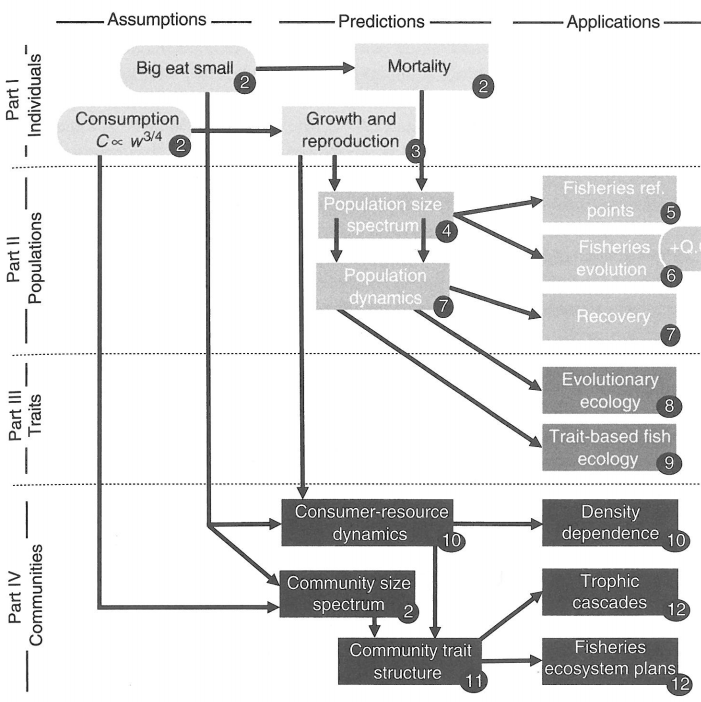
\includegraphics[width=225px]{Fig2} \end{center}

\end{frame}

\begin{frame}{この本を読むにあたって}
\protect\hypertarget{ux3053ux306eux672cux3092ux8aadux3080ux306bux3042ux305fux3063ux3066}{}

\begin{itemize}
\tightlist
\item
  著者が25以上の雑誌に発表した10年以上の成果の集大成である\\
  \vspacesmall
\item
  数式に馴れていない読者のために、概念や原理、結果の説明に重きを置いた\\
  \vspacesmall
\item
  複雑な数式の導出はBoxに示し、Boxを飛ばしても読めるようになっている\\
  \vspacesmall
\item
  図の生成のためのコードはRで書かれており、Web上で公開されている
  \footnote[frame]{https://github.com/Kenhasteandersen/Fish}\\
  \vspacesmall
\item
  始めから最後まで順番に読む必要はない\\
  \vspacesmall
\item
  少なくとも2章の最初の部分を呼んで理論の基本となる前提を理解し、可能であれば3章も合わせて読むことを推奨する
\end{itemize}

\end{frame}

\end{document}
